% 保留全部 IsoFLOP 实测点、拟合线、数值与图例；仅翻译轴题。
\begin{tikzpicture}
\node[anchor=south west,inner sep=0] (plot) at (0,0) {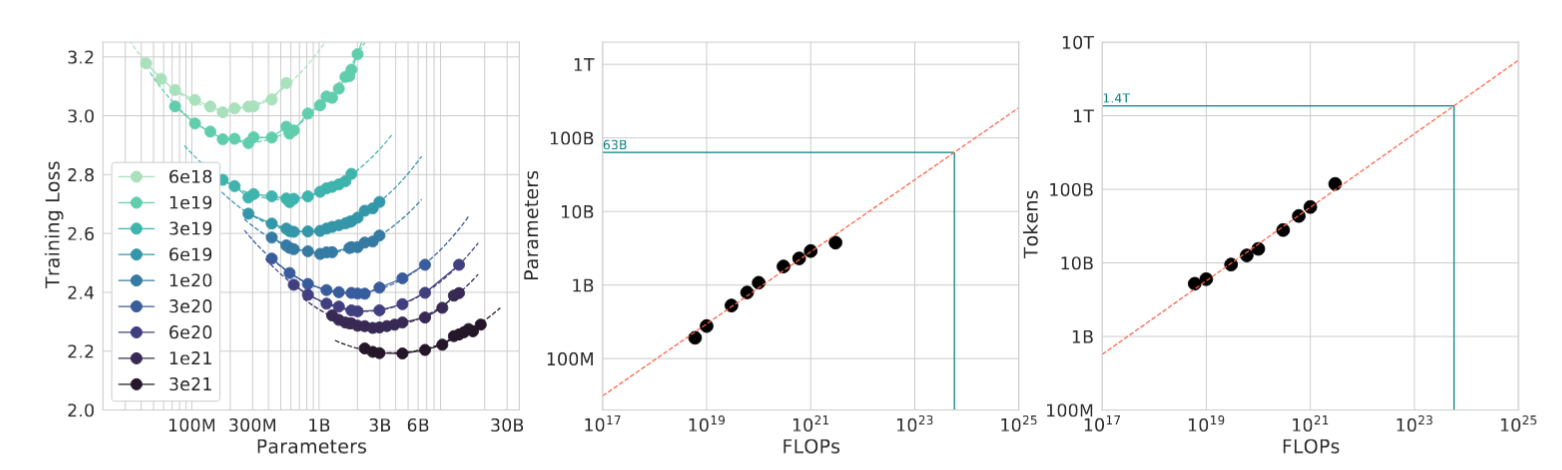
\includegraphics[width=\linewidth]{part1/visuals/isoflop.png}};
\begin{scope}[x={(plot.south east)},y={(plot.north west)},every node/.style={font=\scriptsize,inner sep=0pt}]
\fill[white] (.018,.30) rectangle (.040,.70);
\node[rotate=90] at (.031,.50) {训练损失};
\fill[white] (.331,.30) rectangle (.350,.70);
\node[rotate=90] at (.341,.50) {参数量};
\fill[white] (.654,.32) rectangle (.670,.68);
\node[rotate=90] at (.662,.50) {词元数};
\fill[white] (.12,0) rectangle (.28,.075);
\node at (.20,.028) {参数量};
\end{scope}
\end{tikzpicture}
